\documentclass[12pt]{article}
%Also I made it 12pt

\usepackage[fontset=macnew]{ctex}
\usepackage{physics}
\usepackage{tikz}
\usetikzlibrary{3d,calc,patterns,chains,arrows.meta, positioning}
% \usepackage{tkz-euclide}
\usepackage{amsmath}
\usepackage{upgreek}
\usepackage{amsthm}
\usepackage{amsfonts}

\usepackage{pgfplots}
\pgfplotsset{compat=1.18}

%to add an affiliation line to the the title formatting
\usepackage{authblk}

%Fonts
% \usepackage[no-math]{fontspec} %This allows you to enter (via an IPA kayboard) IPA fonts and other symbols directly into LaTeX. Requires a particular setyp, see below.
\usepackage{libertine} %A font that actually contains many IPA symbols. This is the font you see in the preview to the right.

%to use these fonts, be sure that your typesetting engine is set to "XeLaTeX." In Overleaf, go to the Menu link on the top left (by the Overleaf icon), and under Settings be sure that the Compiler is set to "XeLaTeX." If you accessed this document via the Overleaf Pomona Linguistics template, all of this was already done for you.

%The Pomona Linguistics Paper Template in Overleaf is already set up for this, but you may run into this problem if you start building your own documents.


%%%%%%%%%%%%%%%%%%%%%%%%%%%%%%%%%%%%%%%%%%%%%%%%%%%
%packages for this style of handout-formatting of (sub)section headers 
\usepackage[explicit]{titlesec}
\usepackage{xcolor}

\definecolor{light-gray}{gray}{0.7}
\definecolor{lighter-gray}{gray}{0.85}

\titleformat{\section}
{\normalfont\Large\bfseries}{}{0em}{\colorbox{black}{\parbox{\dimexpr\textwidth-2\fboxsep\relax}{\textcolor{white}{\thesection\quad#1}}}}

\titleformat{\subsection}
{\normalfont\large\bfseries\scshape}{}{0em}{\colorbox{light-gray}{\parbox{\dimexpr\textwidth-2\fboxsep\relax}{\textcolor{black}{\thesubsection\quad#1}}}}

\titleformat{\subsubsection}
{\normalfont\bfseries}{}{0em}{\colorbox{lighter-gray}{\parbox{\dimexpr\textwidth-2\fboxsep\relax}{\textcolor{black}{\thesubsubsection\quad#1}}}}
%%%%%%%%%%%%%%%%%%%%%%%%%%%%%%%%%%%%%%%%%%%%%%%%%%%

%%% This file is the preamble for the Pomona Linguistics LaTeX Paper Template, which is also used for the Quick Reference Guide. If you are brand new to writing with LaTeX, we suggest NOT messing with it, and just writing your paper using the Paper Template. If you are getting more comfortable in LaTeX and want to add packages and commands, this is where you do it (when using this template).

%For stacking text, used here in autosegmental diagrams
\usepackage{stackengine}

%To combine rows in tables
\usepackage{multirow}

%geometry helps manage margins, among other things.
\usepackage[margin=1in]{geometry}

%Gives some extra formatting options, e.g. underlining/strikeout
\usepackage{ulem}

%For putting links into papers, also helps make cross-references in the paper smart references
\usepackage[colorlinks = true,
            linkcolor = blue,
            urlcolor  = blue,
            citecolor = blue,
            anchorcolor = blue]{hyperref} %smarter cross-references, these options turn links blue

%Use package/command below to create a double-spaced document, if you want one. Uncomment BOTH the package and the command (\doublespacing) to create a doublespaced document, or leave them as is to have a single-spaced document.
%\usepackage{setspace}
%\doublespacing 

%paragraph formatting
\usepackage[parfill]{parskip}
\setlength{\parskip}{5pt} %plus 1 minus 1}
\setlength{\parindent}{30pt}
\usepackage{titlesec}

%use for special OT tableaux symbols like bomb and sad face. must be loaded early on because it doesn't play well with some other packages
\usepackage{fourier-orns}

%Basic math symbols 
\usepackage{pifont}
\usepackage{amssymb}

%%%Gives shortcuts for glossing. The use of this package is NOT explained in the Quick Reference Guide, but the documentation is on CTAN for those that are interested. MJKD finds it handy for glossing. (https://ctan.org/pkg/leipzig?lang=en)
\usepackage{leipzig}

%Tables
\usepackage{caption} %For table captions
\usepackage{booktabs} %helps format tables

%For citations and bibliography - as of 9.1.2019 we don't explain citations in this Quick Reference Guide, but Pedro Martin's tutorial does (see links in the Guide).
\usepackage{natbib}

%For OT-style tableaux
\usepackage{ot-tableau}

%highlights text with \hl{text}
\usepackage{color, soul}

%Drawing Syntax Trees
\usepackage[linguistics]{forest}

%This specifies some formatting for the forest trees to make them nicer to look at
\forestset{
  nice nodes/.style={
    for tree={
      inner sep=0pt,
      fit=band,
    },
  },
  default preamble=nice nodes,
}

%% For numbered and glossed examples %%
\usepackage{gb4e}



%Changes the \maketitle command to be smaller and take up less space on a page. 
\makeatletter         
\def\@maketitle{   % custom maketitle 
\noindent {\Large \bfseries \color{black} \@title}  \\ \hrule \noindent \@author \\ \@date  
}

%The code below will draw a circle around a piece of text. This is very useful for drawing attention to a word in a data example. use the command \circled{text} where the argument (`text' here) is what you want to be circled. This is illustrated in the Quick Reference Guide and the Paper Template.

\usepackage{tikz}

\newcommand{\circled}[1]{\begin{tikzpicture}[baseline=(word.base)]
\node[draw, rounded corners, text height=8pt, text depth=2pt, inner sep=2pt, outer sep=0pt, use as bounding box] (word) {#1};
\end{tikzpicture}
}


%%%%%%%%%%%%%%%%%%%%%%%%%%%%%%%%%%%%%%%%%%%%%%%%%%%%%%%%%%%%
%%%%%%%%%%%%%%%%%%%%%%%%%%%%%%%%%%%%%%%%%%%%%%%%%%%%%%%%%%%%

% Useful Ling Shortcuts

\RequirePackage{leipzig}
%\RequirePackage{mathtools} % for \mathrlap

% % % Shortcuts  (borrowed from JZ, I'm still unsure exactly what xspace requires)
\RequirePackage{xspace}
\xspaceaddexceptions{]\}}

%This makes the \emptyset command be a nicer one
\let\oldemptyset\emptyset
\let\emptyset\varnothing
\newcommand{\nothing}{$\emptyset$}

%Not all of these are explained in the Quick Reference Guide, but they are here bc they are relevant to some of our students.
\newcommand{\1}{\rlap{$'$}\xspace}
\newcommand{\0}{\rlap{\textsuperscript{$ˆ{\circ}$}}\xspace}
\newcommand{\Lb}[1]{$\text{[}_{\text{#1}}$ } %A more convenient left bracket
\newcommand{\Rb}[1]{$\text{]}_{\text{#1}}$ } %A more convenient left bracket
\newcommand{\gap}{\underline{\hspace{1.2em}}}
\newcommand{\vP}{\emph{v}P}
\newcommand{\lilv}{\emph{v}}
\newcommand{\Abar}{A$'$-} %A more convenient A-bar notation
\newcommand{\ph}{$\varphi$\xspace} %A more convenient phi
\newcommand{\pro}{\emph{pro}\xspace}
\newcommand{\subs}[1]{\textsubscript{#1}} %A more convenient subscript
%\newcommand{\hd}{$^{\circ}$\xspace} %Symbol for printing head / degree symbol
\newcommand{\spells}{$\Longleftrightarrow$} %spellout arrow for morph spellout rules
% \newcommand{\tr}[1]{\textit{t}\textsubscript{\textit{#1}}} %easy traces with subscript
\newcommand{\supers}[1]{\textsuperscript{#1}}

% Abbreviations for glossing, based on Leipzig
\newleipzig{hab}{hab}{habitual}
\newleipzig{rem}{rem}{remote}
\newleipzig{sm}{sm}{subject marker}
\newleipzig{t}{t}{tense}
\newleipzig{aa}{aa}{anti-agreement}
\newleipzig{pron}{pron}{pronoun}
\newleipzig{rec}{rec}{recent}
\newleipzig{om}{om}{object marker}
%\newleipzig{ipfv}{ipfv}{imperfective}
\newleipzig{asp}{asp}{aspect}
\newleipzig{lk}{lk}{linker}
\newleipzig{pcl}{pcl}{particle}
\newleipzig{stat}{stat}{stative}
\newleipzig{ints}{ints}{intensive}
\newleipzig{ascl}{ascl}{assertive subject clitic}
\newleipzig{nascl}{nascl}{non-assertive subject clitic}
\newleipzig{ta}{ta}{tense and/or aspect}
\newleipzig{assoc}{assoc}{associative marker}
\newleipzig{hon}{hon}{honorific}
%\newleipzig{whprt}{wh}{\wh particle}
\newleipzig{sa}{sa}{subject agreement}
\newleipzig{conj}{conj}{conjunction}
%\newleipzig{loc}{loc}{locative}
\newleipzig{expl}{expl}{expletive}
\newleipzig{rcm}{rcm}{reciprocal marker}
\newleipzig{pers}{pers}{persistive}
%\newleipzig{}{}{} %this is just to copy for when I want to add more

%%%%%%%%%%%%%%%%%%%%%%%%%%%%%%%%%%%%%%%%%%%%%%%%%%%%%%%%%%%%
%%%%%%%%%%%%%%%%%%%%%%%%%%%%%%%%%%%%%%%%%%%%%%%%%%%%%%%%%%%%

%A couple of packages that seemed to prefer being called toward the end of the preamble

%This package provides macros for typesetting SPE-style phonological rules.
\usepackage{phonrule}

%For using Greek letters outside of math mode.
\usepackage{textgreek}


%Random, lets us use the XeLaTeX logo. Not important to the template at all.
\usepackage{metalogo}


%%%%%%%%%%%%
%% This is the end of the PREAMBLE
%%%%%%%%%%%

%MJKD note to future self - this preamble is just the section headers + PomLing formatting, but an ordering paradox between the two files made me combine them and re-order fontspec. *shrug* In future if it needs an update, just take the PomLing formatting file and add in the section headers for handouts.

\newcommand{\rmd}{\mathrm{d}}
\newcommand{\deriv}[2]{\frac{\rmd #1}{\rmd #2}}
\newcommand{\pderiv}[2]{\frac{\partial #1}{\partial #2}}
\newcommand{\dpderiv}[2]{\dfrac{\partial #1}{\partial #2}}
\newcommand{\dderiv}[2]{\dfrac{\rmd #1}{\rmd #2}}

\title{半导体器件}
\author{\href{mailto:lai-wei@whu.edu.cn}{Lai Wei}}
\date{\today}

\begin{document}

\maketitle

\section{半导体的导电特性}

\subsection{本征半导体}

半导体材料具有晶体结构,每个原子核最外层空间的价电子与相邻原子核的价电子形成了共价键结构,对价电子形成约束。常温下有少量的价电子获得外界能量,挣脱束缚而成为自由电子,同时在共价键中留下一个空位子——空穴,这一过程称为激发。

在半导体中同时存在着电子导电和空穴导电。自由电子和空穴都称为载流子。在本征半导体中自由电子和空穴总是成对出现,同时又不断复合。

\subsection{N型半导体和P型半导体}

本征半导体导电能力很低。如果在其中掺入微量的杂质(某种元素),这将使参杂后的半导体(杂志半导体)的导电性能大大增强。

例如在硅晶体中掺入五价元素磷,自由电子是多数载流子,空穴是少数载流体(电子导电是主要导电方式),形成电子型半导体或N型半导体;又如在硅晶体中掺入三价元素硼,空穴是多数载流子,自由电子是少数载流体(空穴导电是主要导电方式),形成空穴型半导体或P型半导体。

\subsection{PN结及其单向导电性}

通常是在一块N型(或P型)半导体的局部再掺入浓度较大的三价(五价)杂质,使其变为P型(或N型)半导体。在P型半导体和N型半导体的交界面就形成了一个特殊的薄层,称为PN结。

当在PN结上加正向电压,即电源正极接卫区,负极接N区时,P区的多数载流子空穴和N区的多数载流子自由电子在电场作用下通过PN结进人对方,两者形成较大的正向电流。此时PN结呈现低电阻,处于导通状态。

当在PN结上加反向电压时,P区和N区的多数載流子受阻,难于通过PN结。但P区的少数载流子自由电子和N区的少数载流子空穴在电场作用下却能通过PN结进人对方,形成反向电流。由于少数载流子数量少,因此反向电流极小。此时PN结呈现高电阻,处于截止状态。

此即为PN结的单向导电性,PN结是各种半导体器件的共同基础。

\section{二极管}

\subsection{基本结构}

将PN结加上相应的电极引线和管壳,就成为二极管。按结构分,二极管有点接触型、面接触型和平面型三类。

\subsection{伏安特性}

二极管具有单向导电性,伏安曲线如下

\begin{figure}[!h]
    \centering
    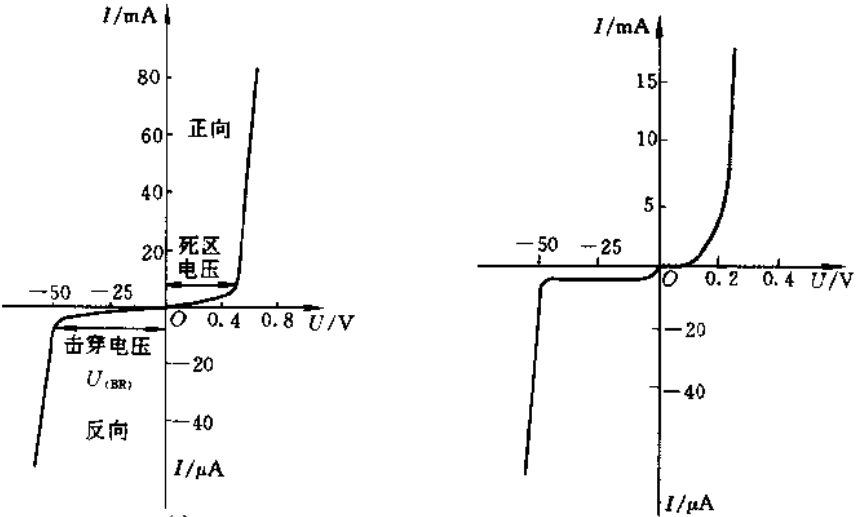
\includegraphics[width=.8\textwidth]{graphics/Screenshot 2025-09-23 at 12.21.48.png}
    \caption{二极管的伏安特性曲线}
\end{figure}

当外加正向电压很低时,正向电流很小,几乎为零。当正向电压超过一定数值后,电流增大很快。这个一定数值的正向电压称为死区电压。

在二极管上加反向电压时,反向电流很小。但当把反向电流加大至某一数值时,反向电流将突然增大。这种现象称为击穿,二极管失去单向导电性。产生击穿时的电压称为击穿电压。

\subsection{主要参数}

\begin{enumerate}
    \item 最大整流电流\(I_{OM}\):二极管长期使用时,允许流过二极管的最大正向平均电流。
    \item 最高反向工作电压\(U_{RWM}\):反向击穿电压\(U_{BR}\)的1/2或1/3为最高反向工作电压。
    \item 反向电流\(I_{RM}\):二极管在反向工作下的电流就是反向电流。
    \item 最高工作频率\(f_M\):二极管工作的上限频率,由PN结的结电容决定。
\end{enumerate}

\section{稳压二极管}

稳压二极管工作于反向击穿区。反向电压在一定范围内变化时,反向电流很小。当反向电压增高到击穿电压时,反向电流突然剧增,稳压二极管反向击穿。此后,电流虽然在很大范围内变化,但稳压二极管两端的电压变化很小。利用这一特性,稳压二极管在电路中能起稳压作用。稳压二极管与一般二极管不一样,它的反向击穿是可逆的。当去掉反向电压之后,稳压二极管又恢复正常。但是,如果反向电流超过允许范围,稳压吧二极管将会发生热击穿而损坏。

稳压二极管的主要参数有

\begin{enumerate}
    \item 稳定电\(U_Z\):稳压管正常工作(反向击穿)时管两端的电压;
    \item 电压温度系数\(\alpha_U\)
    \item 稳定电流、最大稳定电流;
    \item 动态电阻\(r_z = \dfrac{\Delta U_Z}{\Delta I_Z}\):越小,曲线越陡,稳压性能越好;
    \item 最大允许耗散功率\(P_{ZM} = U_Z I_{ZM}\):管子不发生热击穿的最大功率损耗。
\end{enumerate}

\section{双极型二极管}

双极型二极管又称三极管,通常简称为晶体管。

\subsection{基本结构}

晶体管的结构,目前最常见的有平面型和合金型两类。硅管主要是平面型,锗管都是合金型。

不论平面型或合金型,都分成NPN或PNP三层,因此又把晶体管分为NPN型和PNP型两类。

每一类都分成基区、发射区和集电区,分别引出基极B、发射极E和集电极C。每一类都有两个PN结。基区和发射区之间的结称为发射结,基区和集电区之同的结称为集电结。

\begin{figure}[!h]
    \centering
    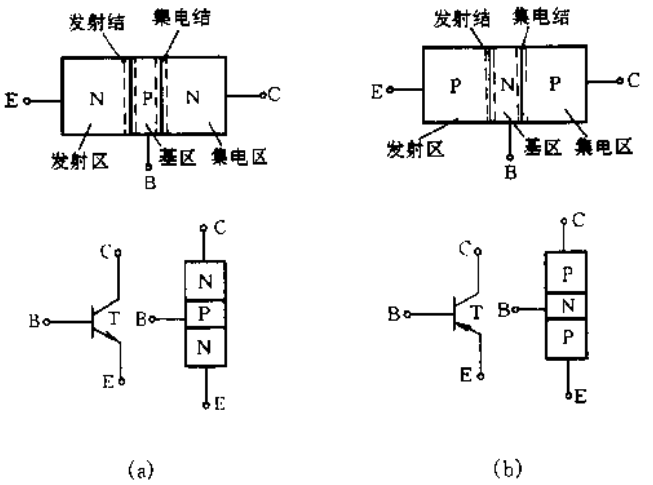
\includegraphics[width=.6\textwidth]{graphics/Screenshot 2025-09-23 at 12.22.38.png}
    \caption{晶体管的结构示意图和表示符号}
\end{figure}

\subsection{电流分配和放大原理}

\begin{figure}[!h]
    \centering
    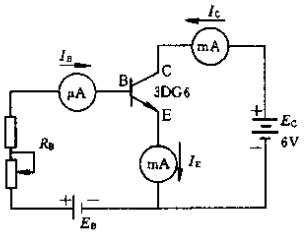
\includegraphics[width=.25\textwidth]{graphics/Screenshot 2025-09-28 at 06.44.14.png}
    \caption{晶体管电流放大的实验电路}
\end{figure}

有以下结论:

\begin{enumerate}
    \item $I_E = I_C + I_B$,符合基尔霍夫电路
    \item \(I_C\)和\(I_E\)\(I_B\)大得多,\(I_C\)与\(I_B\)的比值为
        \begin{equation}
        \beta = \frac{\Delta I_C}{\Delta I_E}
        \end{equation}式中,\(\beta\)称为\emph{动态电流(交流)放大系数}。
    \item 当$I_B = 0$(将基极开路)时,\(I_C = I_CEO\)
    \item 要使晶体管起放大作用,发射结必须正向偏置,而集电结必须反向偏置。
\end{enumerate}

NPN型:集电极电位最高,发射极电位最低;PNP型:发射极电位最高,集电极电位最低。

NPN型硅管:基极电位比发射极电位大约高0.6 -- 0.7V;PNP型锗管:基极电位比发射极电位大约低0.2 -- 0.3V。

\begin{table}[!h]
    \centering
    \begin{tabular}{c|c|c|c}
    \hline 管脚 & 1 & 2 & 3 \\
    \hline 电位/V & 4 & 3.4 & 9 \\
    \hline 电极 & B & E & C \\
    \hline 类型 & \multicolumn{3}{|c}{ NPN 型 } \\
    \hline 材料 & \multicolumn{3}{|c}{ 硅管 } \\
    \hline
    \end{tabular}
\end{table}

\begin{table}[!h]
    \centering
    \begin{tabular}{c|c|c|c}
    \hline 管脚 & 1 & 2 & 3 \\
    \hline 电位/V & -6 & -2.3 & -2 \\
    \hline 电极 & C & B & E \\
    \hline 类型 & \multicolumn{3}{|c}{ PNP 型 } \\
    \hline 材料 & \multicolumn{3}{|c}{ 锗管 } \\
    \hline
    \end{tabular}
\end{table}

\subsection{特性曲线}


\end{document}
